\documentclass[12pt]{article}
\usepackage[utf8]{inputenc}
\usepackage[spanish]{babel}
\usepackage{siunitx}
% ---------------------------------------------------
% 						FONT 
% ---------------------------------------------------

\usepackage{cmbright}								% Font
\documentclass{article}
\usepackage{siunitx}
\usepackage{hyperref} % LINKS
\usepackage{caption}
\decimalpoint
\usepackage{mathtools}
\usepackage{amsmath}
\usepackage{amsthm}
\usepackage{amssymb}
\usepackage{graphicx}
\usepackage[margin=0.9in]{geometry}
\usepackage{fancyhdr}
\usepackage[inline]{enumitem}
\usepackage{float}
\usepackage{cancel}
\usepackage{bigints}
\usepackage{color}
\usepackage{xcolor}
\usepackage{listingsutf8}
\usepackage{algorithm}
\usepackage{tocloft}
\usepackage[none]{hyphenat}
\usepackage{graphicx}
\usepackage{grffile}
\usepackage{tabularx}
\usepackage[nottoc,notlot,notlof]{tocbibind}
\usepackage{times}
\usepackage{color}
\definecolor{gray97}{gray}{.97}
\definecolor{gray75}{gray}{.75}
\definecolor{gray45}{gray}{.45}
\renewcommand{\cftsecleader}{\cftdotfill{\cftdotsep}}
\pagestyle{fancy}
\setlength{\headheight}{15pt} 
\lhead{Práctica 2: Sensores Resistivos: Potenciométrico}
\rhead{\thepage}
\lfoot{ESCOM-IPN}
\renewcommand{\footrulewidth}{0.5pt}
\setlength{\parskip}{0.5em}
\newcommand{\ve}[1]{\overrightarrow{#1}}
\newcommand{\abs}[1]{\left\lvert #1 \right\lvert}
\date{ 01 de Junio 2018}
\title{Potenciometrico}
\author{Instrumentacion}

\definecolor{pblue}{rgb}{0.13,0.13,1}
\definecolor{pgreen}{rgb}{0,0.5,0}
\definecolor{pred}{rgb}{0.9,0,0}
\definecolor{pgrey}{rgb}{0.46,0.45,0.48}
\lstset{tabsize=1}
\usepackage{wrapfig}

\usepackage{listings}
\lstset{ frame=Ltb,
framerule=0pt,
aboveskip=0.5cm,
framextopmargin=3pt,
framexbottommargin=3pt,
framexleftmargin=0.4cm,
framesep=0pt,
rulesep=.4pt,
backgroundcolor=\color{gray97},
rulesepcolor=\color{black},
%
stringstyle=\ttfamily,
showstringspaces = false,
basicstyle=\small\ttfamily,
commentstyle=\color{gray45},
keywordstyle=\bfseries,
%
numbers=left,
numbersep=15pt,
numberstyle=\tiny,
numberfirstline = false,
breaklines=true,
}

% minimizar fragmentado de listados
\lstnewenvironment{listing}[1][]
{\lstset{#1}\pagebreak[0]}{\pagebreak[0]}

\lstdefinestyle{consola}
{basicstyle=\scriptsize\bf\ttfamily,
backgroundcolor=\color{gray75},
}

\lstdefinestyle{Java}
{language=Java,
}

%%%%%%%%%%%%%%%%%%%%%

\lstdefinestyle{customc}{
  belowcaptionskip=1\baselineskip,
  breaklines=true,
  frame=L,
  xleftmargin=\parindent,
  language=C,
  showstringspaces=false,
  basicstyle=\footnotesize\ttfamily,
  keywordstyle=\bfseries\color{green!40!black},
  commentstyle=\itshape\color{purple!40!black},
  identifierstyle=\color{blue},
  stringstyle=\color{orange},
}

\lstdefinestyle{customasm}{
  belowcaptionskip=1\baselineskip,
  frame=L,
  xleftmargin=\parindent,
  language=[x86masm]Assembler,
  basicstyle=\footnotesize\ttfamily,
  commentstyle=\itshape\color{purple!40!black},
}

\lstset{escapechar=@,style=customc}

% Ayuda para el formato de las tablas
\usepackage{array}
% Se declara un nuevo tipo de columna para alinear de manera:
% -Horizontal
\newcolumntype{P}[1]{>{\centering\arraybackslash}p{#1}}
% -Vertical
\newcolumntype{M}[1]{>{\centering\arraybackslash}m{#1}}

% Indica la separacion entre las columnas de una tabla
\setlength{\tabcolsep}{10pt} % Default value: 6pt
% Indica el padding inferior y superior de las celdas de una tabla
\renewcommand{\arraystretch}{1.8} % Default value: 1

\usepackage{longtable}
%Permite crear columnas en el documento
\usepackage{multicol} 
\usepackage{color}
\usepackage{comment}
\newcommand{\tabitem}{~~\llap{\textbullet}~~}
\newcommand{\subtabitem}{~~~~\llap{\textbullet}~~}

\bibliographystyle{IEEEtran}
\begin{document}
		\begin{titlepage}
			\begin{center}
				
				% Upper part of the page. The '~' is needed because \\
				% only works if a paragraph has started.
				
				\noindent
				\begin{minipage}{0.5\textwidth}
					\begin{flushleft} \large
						\includegraphics[width=0.5\textwidth]{../ipn.png}
					\end{flushleft}
				\end{minipage}%
				\begin{minipage}{0.55\textwidth}
					\begin{flushright} \large
						\includegraphics[width=0.4\textwidth]{../escom.png}
					\end{flushright}
				\end{minipage}
				
				\textsc{\LARGE Instituto Politécnico Nacional}\\[0.5cm]
				
				\textsc{\Large Escuela Superior de Cómputo}\\[1cm]
				
				% Title
				
				{ \huge Práctica 2: Sensores Resistivos: Potenciométrico \\[1cm] }
				
				{ \Large Unidad de aprendizaje: Instrumentación} \\[1cm]
				
				{ \Large Grupo: 3CM4 } \\[1cm]
				
				\noindent
				\begin{minipage}{0.5\textwidth}
					\begin{flushleft} \large
						\emph{Integrantes:}\\
						
						\begin{tabular}{ll}
						Aguilar Herrera Arianna Itzamina \\
					    Nicolás Sayago Abigail\\
					    Ramos Diaz Enrique \\
					\end{tabular}
					\end{flushleft}
				\end{minipage}%
				\begin{minipage}{0.5\textwidth}
					\begin{flushright} \large
						\emph{Profesor(a):} \\
						Tellez Barrera Juan Carlos  \\
					\end{flushright}
				\end{minipage}
				
				\vfill
				
				% Bottom of the page
				{\large Fecha de entrega: 16 de Septiembre de 2018}
			\end{center}
		\end{titlepage}
	
	\tableofcontents
	\newpage
	
	% /////////////////////////////////////////////////////////////////////
	%							INTRODUCCION
	% ////////////////////////////////////////////////////////////////////
	\section{Introducción}
	    \subsection{Potenciómetro}
    	Es un resistor eléctrico con un valor de resistencia variable y generalmente ajustable manualmente. Los potenciómetros tienen tres terminales y se suelen utilizar en circuitos de corriente baja, para circuitos de mayor corriente se utilizan los reóstatos. En muchos dispositivos eléctricos los potenciómetros son los que establecen el nivel de salida. Por ejemplo, en un altavoz, el potenciómetro ajusta el volumen; en un televisor o un monitor de ordenador se puede utilizar para controlar el brillo.
    	El valor de un potenciómetro viene expresado en ohmios (símbolo $\Omega$) como las resistencias, y ese valor corresponde siempre es la resistencia máxima que puede llegar a tener. El mínimo valor lógicamente es cero. Por ejemplo, un potenciómetro de 5 kΩ puede tener una resistencia variable con valores entre 0 Ω y 5000 Ω.
    	\begin{figure}[h!]
                \centering
                \includegraphics[width=0.55\textwidth]{Practica2/images/Potenciometro.jpg}
            \end{figure}
        \subsection{Amplificador no inversor}
        En un op-amp ideal, la ganancia del amplificador no inversor está dada por:
        $$
            \frac{V_{out}}{V_{in}}=1+\frac{R_{f}}{R_{1}}
        $$
        \begin{figure}[h!]
                \centering
                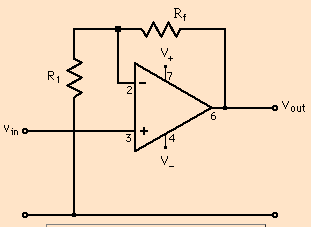
\includegraphics[scale=0.55]{Practica2/images/Ai.jpg}
            \end{figure}

    
	% /////////////////////////////////////////////////////////////////////
	%							DESARROLLO
	% ////////////////////////////////////////////////////////////////////
	\newpage
	\section{Desarrollo}
		\subsection{Esquema del circuito}
		% E N R I K E
		\begin{figure}[h!]
                \centering
                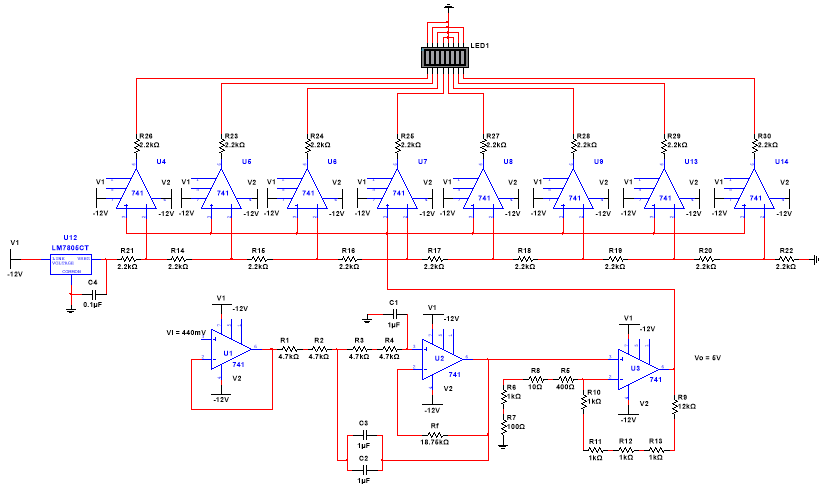
\includegraphics[width=0.75\textwidth]{Practica2/images/circuito.PNG}
            \end{figure} 
        
        \subsection{Circuito cableado}
        \begin{figure}[h!]
                \centering
                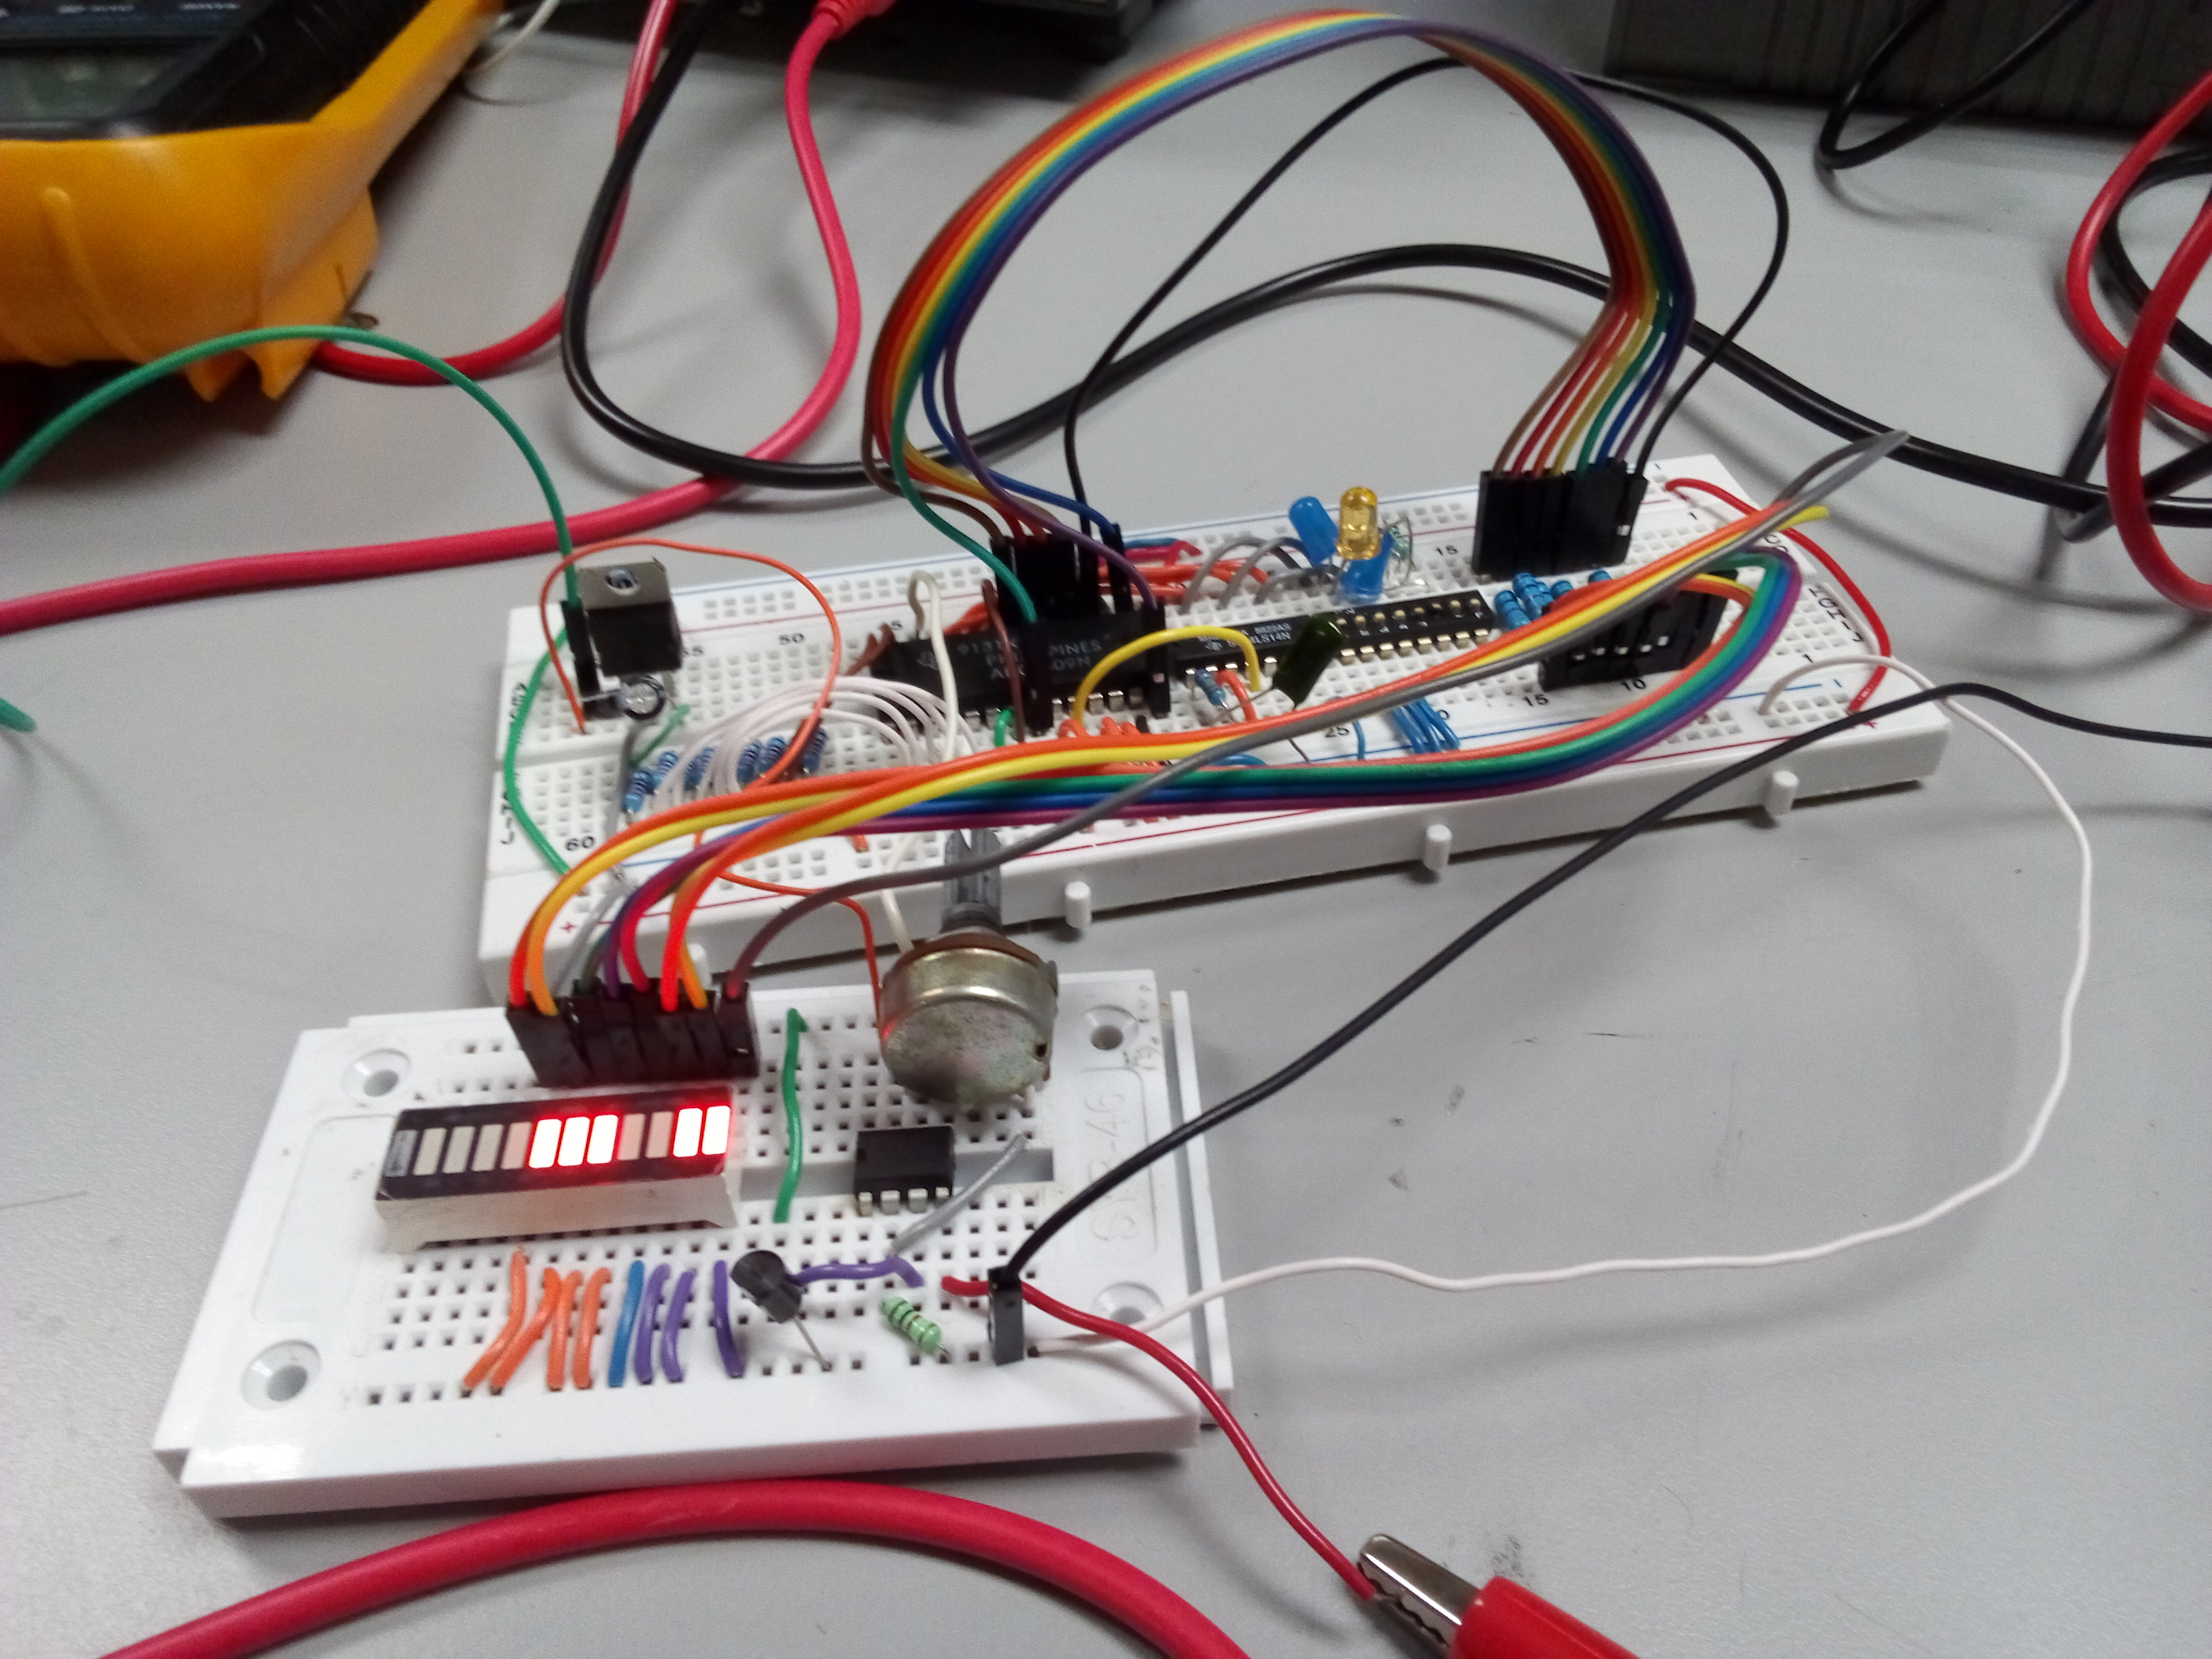
\includegraphics[width=0.7\textwidth]{Practica2/images/circuito4.jpg}
            \end{figure} 
        \newpage
		\subsection{Funcionamiento}
        % A R I
        Conforme se va moviendo el cursor del potenciómetro, va cambiando el voltaje del potenciómetro, y por consecuencia, el de salida, cada voltaje tiene su correspondiente valor en ángulos (según la inclinación del cursor), la tabla de mediciones será expuesta más adelante en el reporte, también se puede observar el ángulo correspondiente en la página creada para ello, igualmente explicada más adelante. 
        
        El diseño de la primera etapa se realizo en serie con una resistencia de $10k\Omega$ para que no existan problemas al momento de reducir el voltaje del potenciómetro de $2k\Omega$ a 0V, así la corriente máxima del circuito tan solo subirá a 1.2mA (aplicando ley de Ohm).
        
        El regulador de voltaje LM7812 es para tener una entrada constante de 12 V, para toda fuente de alimentación. El amplificador no inversor esta diseñado para tener una entrada de 2V, que es el voltaje máximo del potenciómetro, y amplificarla para obtener una salida de 5V constantes (más adelante se explica la función del preset).
		\subsection{Cálculos}
        % E N R I K E
        \subsubsection{Primera Etapa. Potenciómetro.}
        En primer lugar, seleccionamos un valor para la intensidad de la primera parte del circuito, antes de enviar el voltaje de salida del potenciómetro al amplificador operacional.
        
        Nos inclinamos por una intensidad de $I = 1 mA$, que será la misma para todos los componentes de esta etapa.
        
        Ahora seleccionamos el valor en ohms de nuestro potenciómetro, el cuál será de $2k\Omega$ para evitar obtener un voltaje de la fuente demasiado alto.

        Entonces, tenemos:\\
        Intensidad = $1mA$\\
        Potenciómetro = $2k\Omega$
        
        Empleando la ley de Ohm $V = IR$, calculamos el voltaje $V_{o}$ del potenciómetro:
        $$V_{o} = (1 mA)(2k\Omega) = 2 V$$
        
        Ahora, debemos proponer un valor de voltaje para nuestra fuente, ya sea de 5V o de 12V. Nuestra elección fue una fuente de $V_{CC} = 12V$, por lo que debemos de restar el voltaje $V_{o}$ del potenciómetro al de la fuente para obtener el voltaje y valor de la resistencia restante:
        
        $$V_{R} = V_{CC} - V_{o} = 12V - 2V = 10V$$
        
        Ahora bien, solo nos queda por calcular la resistencia restante, por medio de la ley de Ohm:
        
        $$R = \frac{V_{R}}{I} = \frac{10 V}{1 mA} = 10k\Omega$$
        
        Quedando el diseño del circuito de la siguiente manera:\\
        Intensidad = $1mA$\\
        Potenciómetro = $2k\Omega$\\
        Resistencia = $10k\Omega$\\
        Voltaje Fuente = $12 V$
        
        \subsubsection{Segunda Etapa. Amplificador No Inversor.}
        \begin{enumerate}
        \item Definimos la ganancia de voltaje $A_{CL}$, donde el voltaje de entrada es de $V_{o}= 2 V$, que es del potenciometro, y el voltaje de salida deseado sera de $V_{o}'= 5 V$
        		
        		Aplicando las fórmulas del Amplificador No Inversor tenemos:

        				$$ A_{CL} = \frac{V_{o}'}{V{o}} = \frac{5 V}{2 V} = 2.5 $$
        				
        				
        	\item Ahora, utilizamos otra formula que igualaremos con la ecuación anterior:
        	
        	$$ A_{CL} =
        				2.5 = 1 + \frac{R_{f}}{R_{i}} $$
        				
            \item Comenzamos a operar en ella. Pasamos el uno restando al otro lado de la igualdad:
            
            $$ 1.5 = \frac{R_{f}}{R_{i}} $$
        	
        	\item Como vemos, obtuvimos una única ecuación pero con 2 incógnitas. Matemáticamente es imposible solucionar esto. Para evitar quedarnos estancados proponemos un valor para cualquiera de las resistencias. En esta caso elegimos $R_{f} = 15K\Omega$
        	\\
        	$$ 1.5 = \frac{15K\Omega}{R_{i}} $$
            
            \item Pasando dividiendo, obtenemos $R_{i}$
            \\
            $$ R_{i} = \frac{15K\Omega}{1.5} = 10K\Omega $$
            
            \item Los valores de las resistencias son: $R_{i} = 10K\Omega$ y $R_{f} = 15K\Omega$
        	
        	\end{enumerate}

        
        
		\subsection{Ajuste de valores}
        % A R I
        Gracias a los cálculos realizados en la primera y segunda etapa se determinaron los valores necesarios para los componentes del circuito, sin embargo, debemos tomar en cuenta que el circuito, siempre y cuando se aplique bajo las mismas condiciones, pueda llevarse a cabo en cualquier lugar. 
        
        En esta práctica no hubo problema con las resistencias, pues en los cálculos se encontraron valores comerciales, por lo que, el menos para las resistencias no se tuvo que hacer algún ajuste. 
        
        Sin embargo, no solo las resistencias pueden ser ajustadas, como se mencionó, en cualquier lugar, bajo las mismas condiciones, debe funcionar, por lo que, primeramente, hay que garantizar que el voltaje de entrada sea de 12V constantes, para no alterar de modo alguno los cálculos de la primera etapa. Para ello, se utilizó un regulador de voltaje LM7812, pues si solo se depende de la fuente de voltaje, no todas darán ese valor exacto.
        
        Ahora, otro ajuste necesario es garantizar una salida de 5V, pues en caso contrario, se alteraría el resultado esperado, pues no siempre se cumpliría la tabla de valores, que más adelante se mostrará. 
        
        En este caso la desviación que se propuso fue utilizar dos componentes en serie para $R_i$ en el diseño del amplificador no inversor; una resistencia de $1 k\Omega$ y un preset de $10 k\Omega$, para ir ajustando el valor de éste último hasta obtener en $V_{o}'$ el valor deseado de 5V exactos.

        
        
        
        
        
	% /////////////////////////////////////////////////////////////////////
	%							MEDICIONES
	% ////////////////////////////////////////////////////////////////////
	\section{Mediciones}
		\begin{itemize}
			\item \textbf{Ganancia}
			
			    Inicial = 2.5
			    
			    Ajustada = 2.722
			\item \textbf{Voltaje de salida sin ajustar}
			    
			    Mínimo = $10 mV$
			    
			    Máximo = $4.66 V$
			\item \textbf{Voltaje de salida ajustado}
			    
			    Mínimo = $13 mV$
			    
			    Máximo = $5.0048 V$
			    
			\item \textbf{Error}
			
			    $\bigtriangleup$ Error Ganancia = 2.722 - 2.5 = 0.222
			    
			     $\bigtriangleup$ Error Voltaje Mínimo = 0.013 - 0.01 = 0.003
			     
			    $\bigtriangleup$ Error Voltaje Máximo = 5.0048 - 4.66 = 0.3448
		\end{itemize}
	
	% /////////////////////////////////////////////////////////////////////
	%							APLICACIÓN
	% ////////////////////////////////////////////////////////////////////
	\section{Aplicación: Potangle}
		\subsection{Funcionamiento}
            La aplicación que se le dio fue la medición de ángulos según la posición del cursor del potenciómetro. Se realizo una escala en un pedazo de cartón en donde están expresados los ángulos en grados. Posteriormente se recorto un agujero en donde colocamos el potenciómetro de forma horizontal (con sus tres patas hacia abajo y el cursor de frente).
            
            Para una mejor medición y visualización del ángulo en que se encuentra el curso del potenciómetro, colocamos un pedazo largo de papel para que tomara la función de aguja indicadora de ángulo.
            
            El rango de medición en grados es de 20 a 180 grados.
            
            El rango de medición en volts es de 0.013 a 3.0051 volts.
            
            Para determinar la resolución, debido a que nuestros valores de grados y volts no aumentan de forma constante, se opto por realizar una aproximación polinomial a un polinomio de grado 8 para obtener una mayor exactitud, y obtener una función que nos facilite el calculo y medición de voltaje para cualquier valor de ángulo dentro del rango establecido.
            
            \begin{figure}[h!]
                \centering
                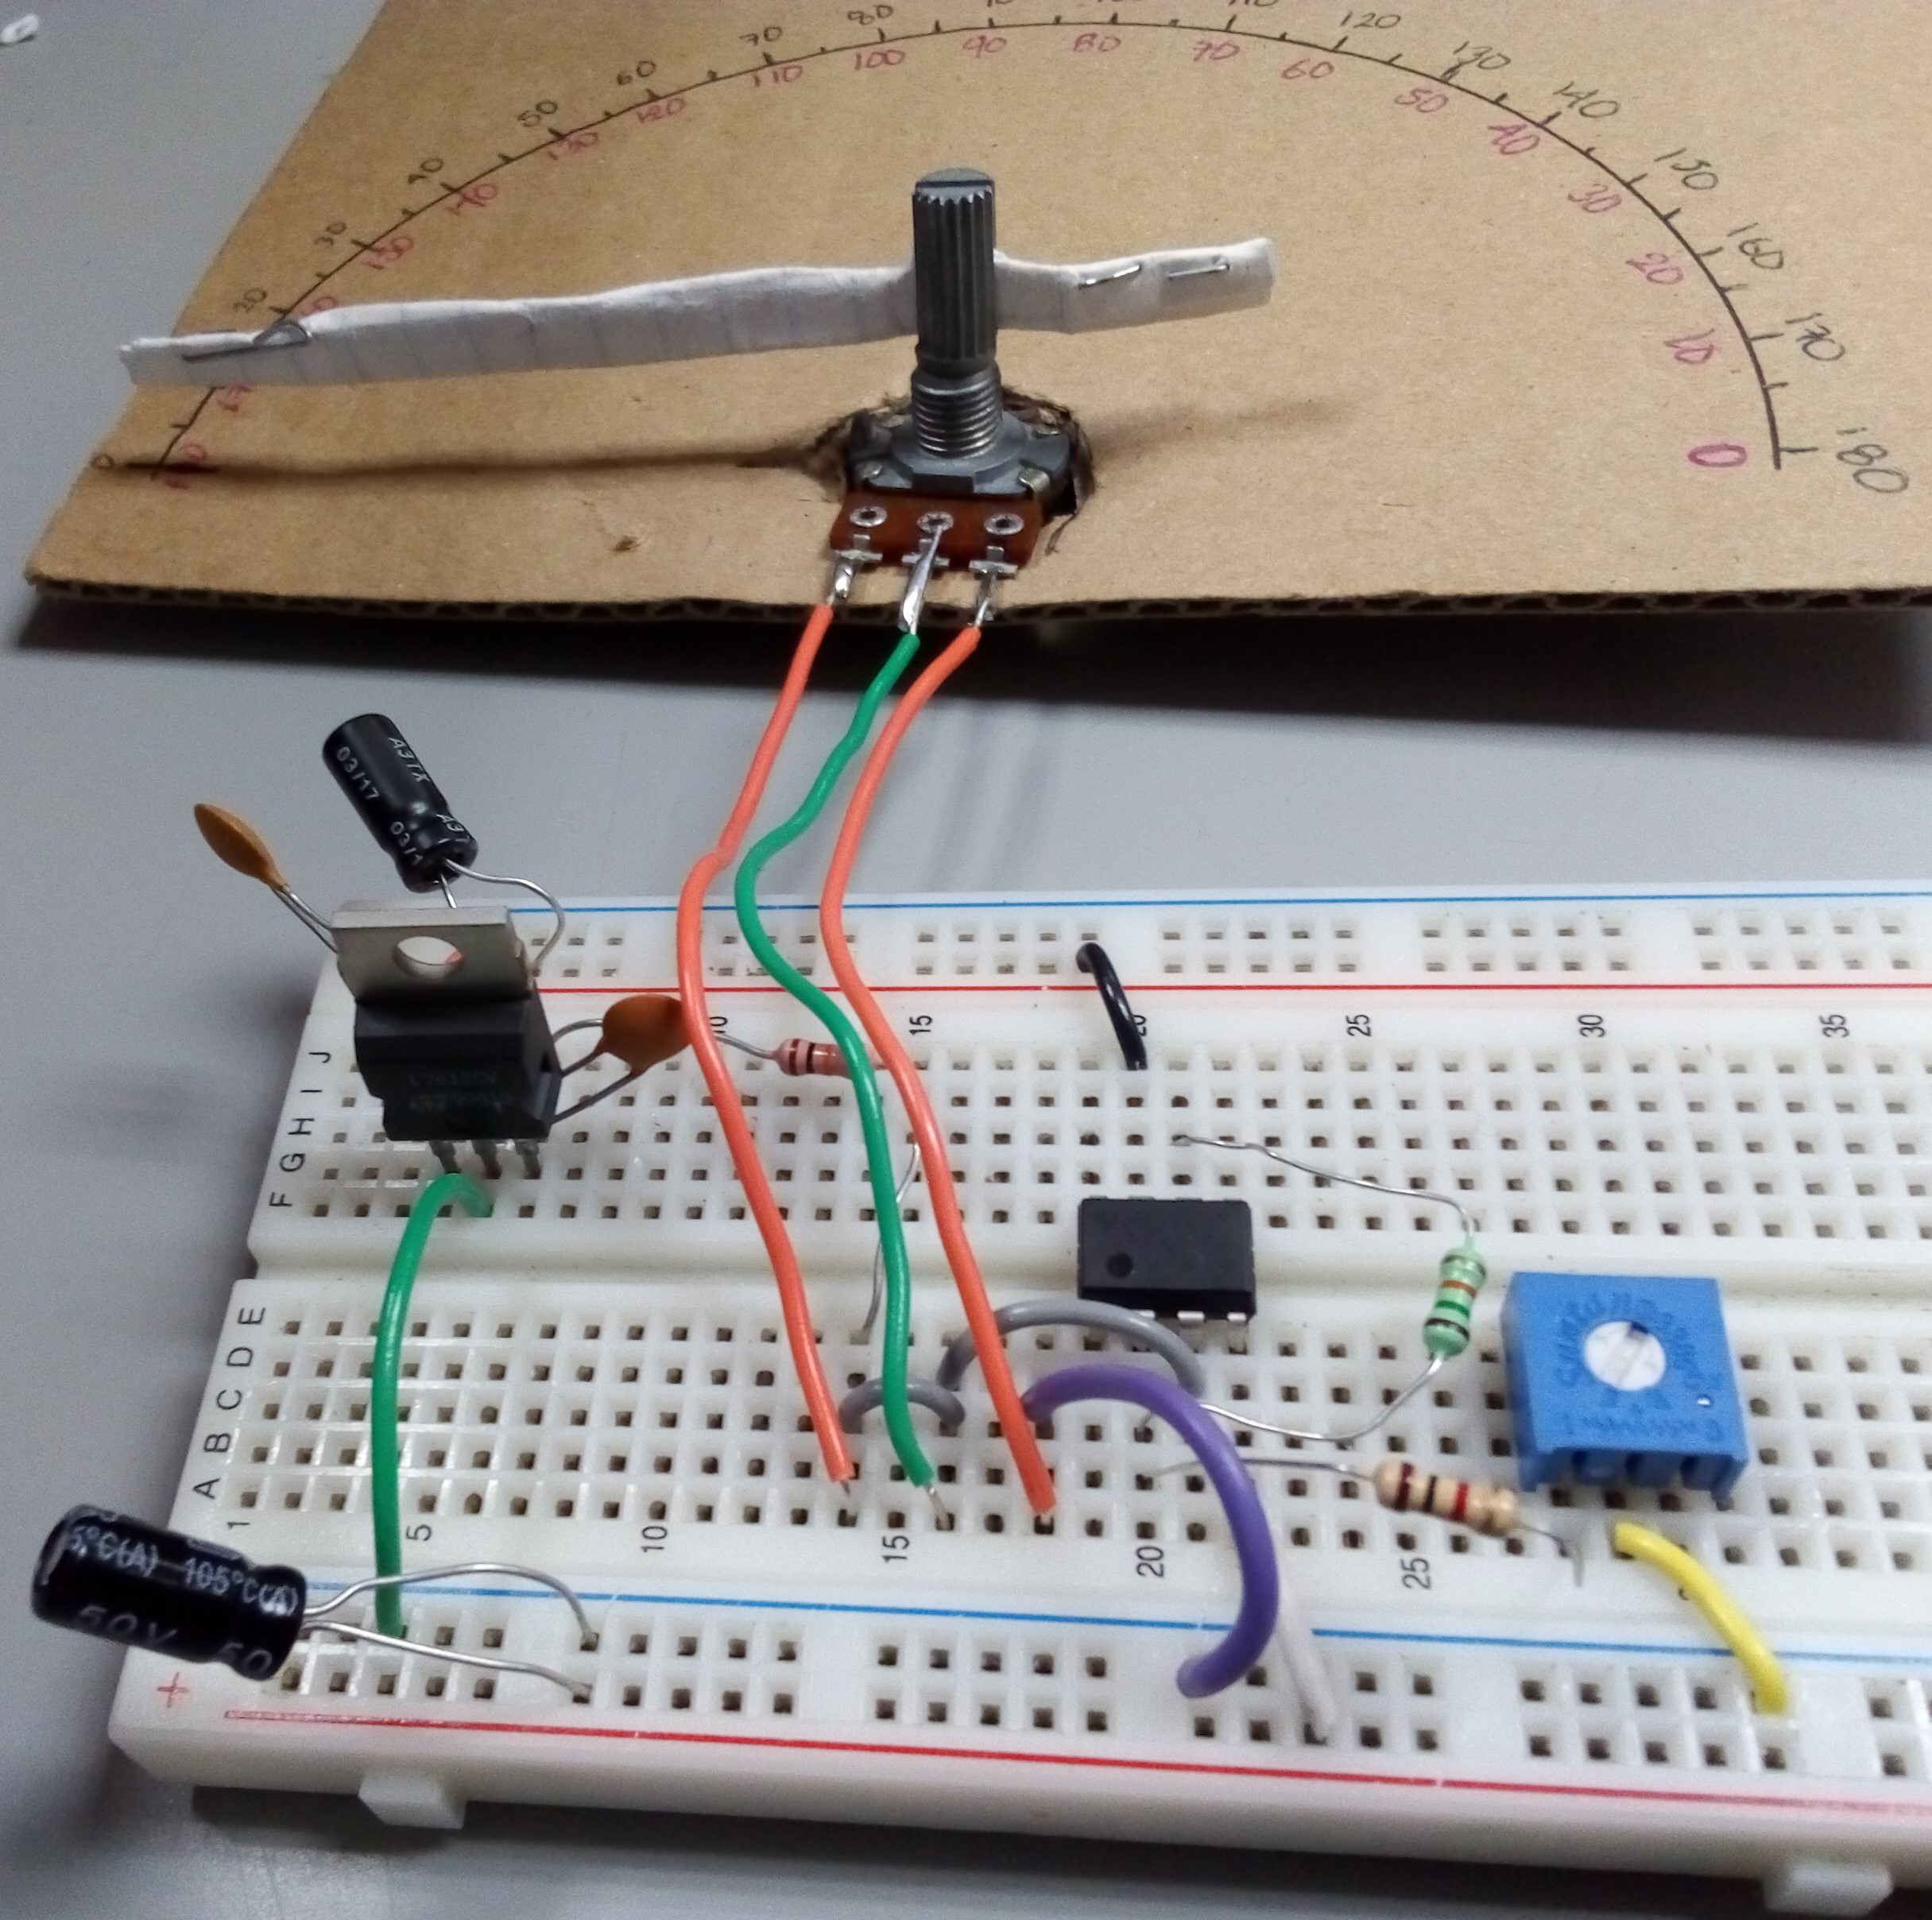
\includegraphics[width=0.7\textwidth]{Practica2/images/potangle3.jpg}
            \end{figure} 
            \begin{figure}[h!]
                \centering
                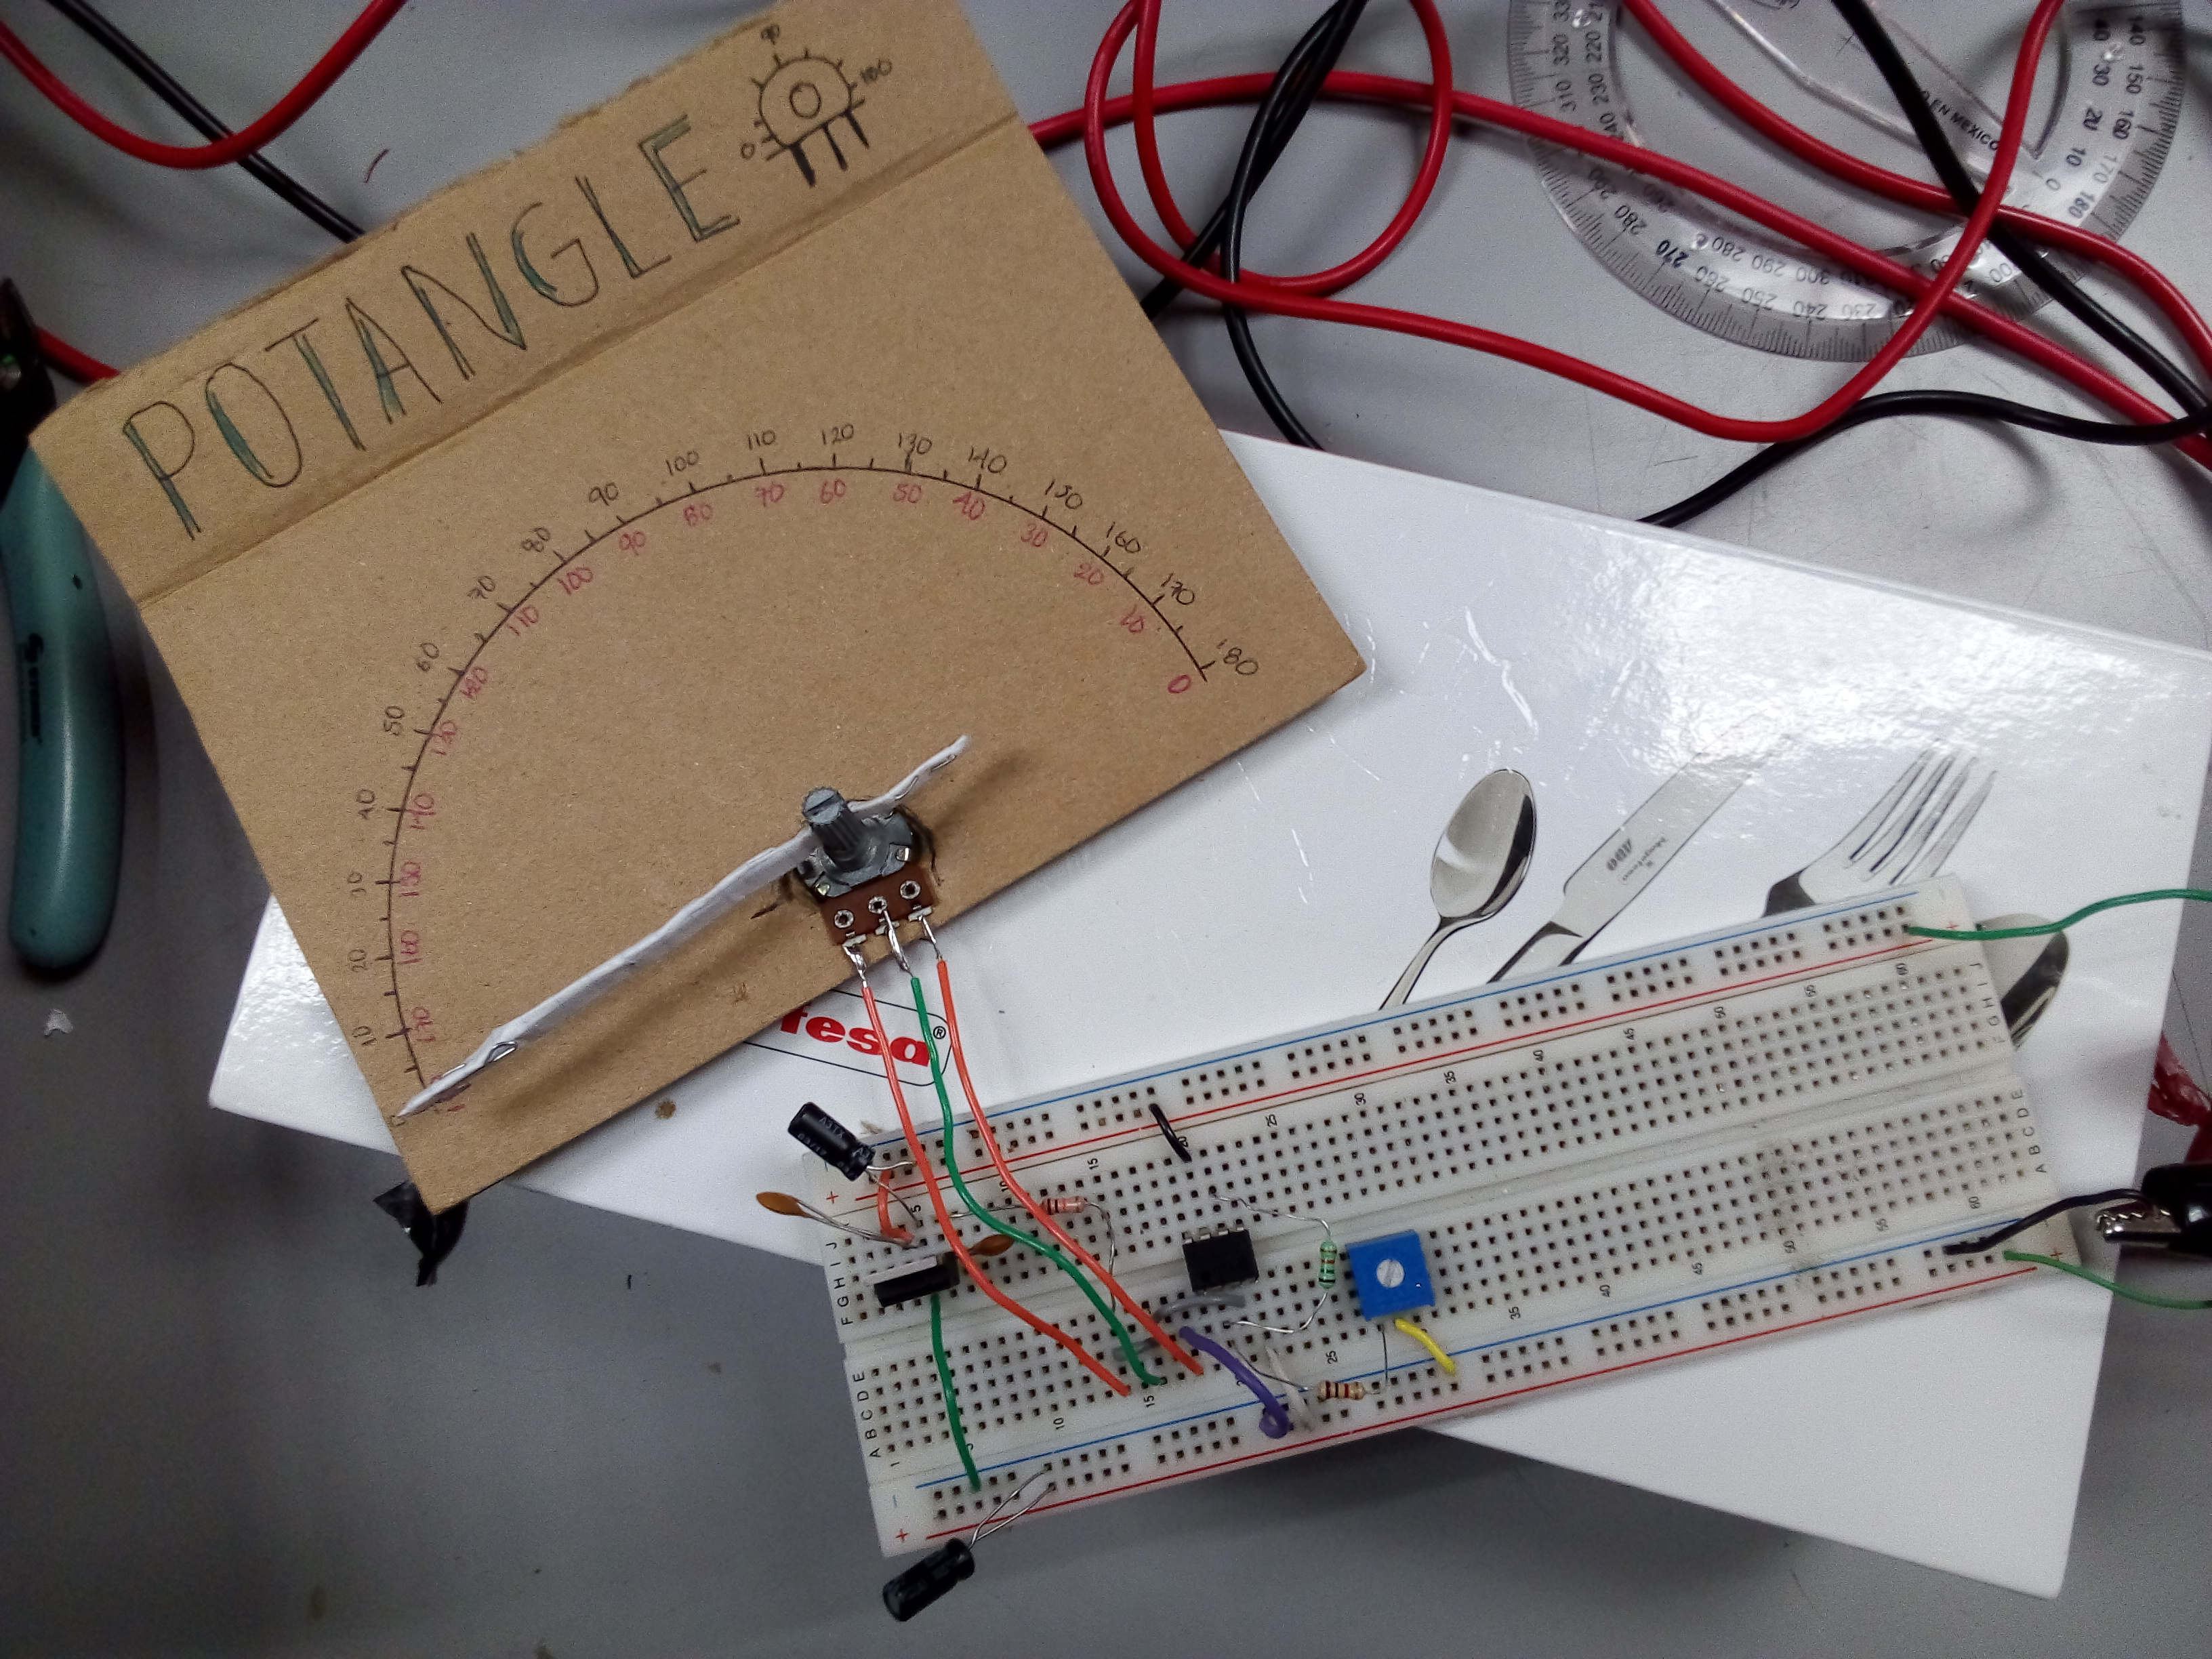
\includegraphics[width=0.7\textwidth]{Practica2/images/potangle.jpg}
            \end{figure}
            

		\subsection{Tabla de valores y gráfica}
		\begin{figure}[h!]
                \centering
                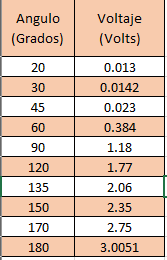
\includegraphics[width=0.3\textwidth]{Practica2/images/medidas.PNG}
            \end{figure}
        \newpage
        El polinomio aproximado a los valores medidos es:

	    \begin{figure}[h!]
	    \centering
                \subfigure{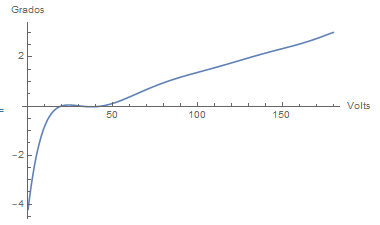
\includegraphics[scale=1.1]{Practica2/images/polinomio.PNG}
                \caption*{\textbf{Grado 8: }$y = -4.20146 + 0.576209 x - 0.0303426 x^2 + 0.000803682x^3 -   0.0000118802 x^4 + 
                1.03454\times10^{-7} x^5 - 5.28161\times10^{-10} x^6 +   1.46335\times10^{-12} x^7 - 1.69911\times10^{-15} x^8$}}
            \end{figure}
        

        En donde:
        
        y son los volts
        
        x son los grados
        
        Así, este polinomio describirá la resolución de la medición, e incluso, nos ayudara a calcular cualquier valor que este dentro del rango de voltaje y dentro del rango de grados que ya establecimos:\\

        Por ejemplo, para hallar el voltaje a 100 grados:
        
        $V = -4.20146 + 0.576209 (100) - 0.0303426 (100)^2 + 0.000803682 (100)^3 -   0.0000118802 (100)^4 + 1.03454\times10^{-7} (100)^5 - 5.28161\times10^{-10} (100)^6 +   1.46335\times10^{-12} (100)^7 - 1.69911\times10^{-15} (100)^8 = 1.37834 V$
        
        Por lo tanto, 1.37 V en 100 grados
        \\
        \\
        \newpage
        \textbf{Medida a 90 grados = 1.18 V}
        \begin{figure}[h!]
                \centering
                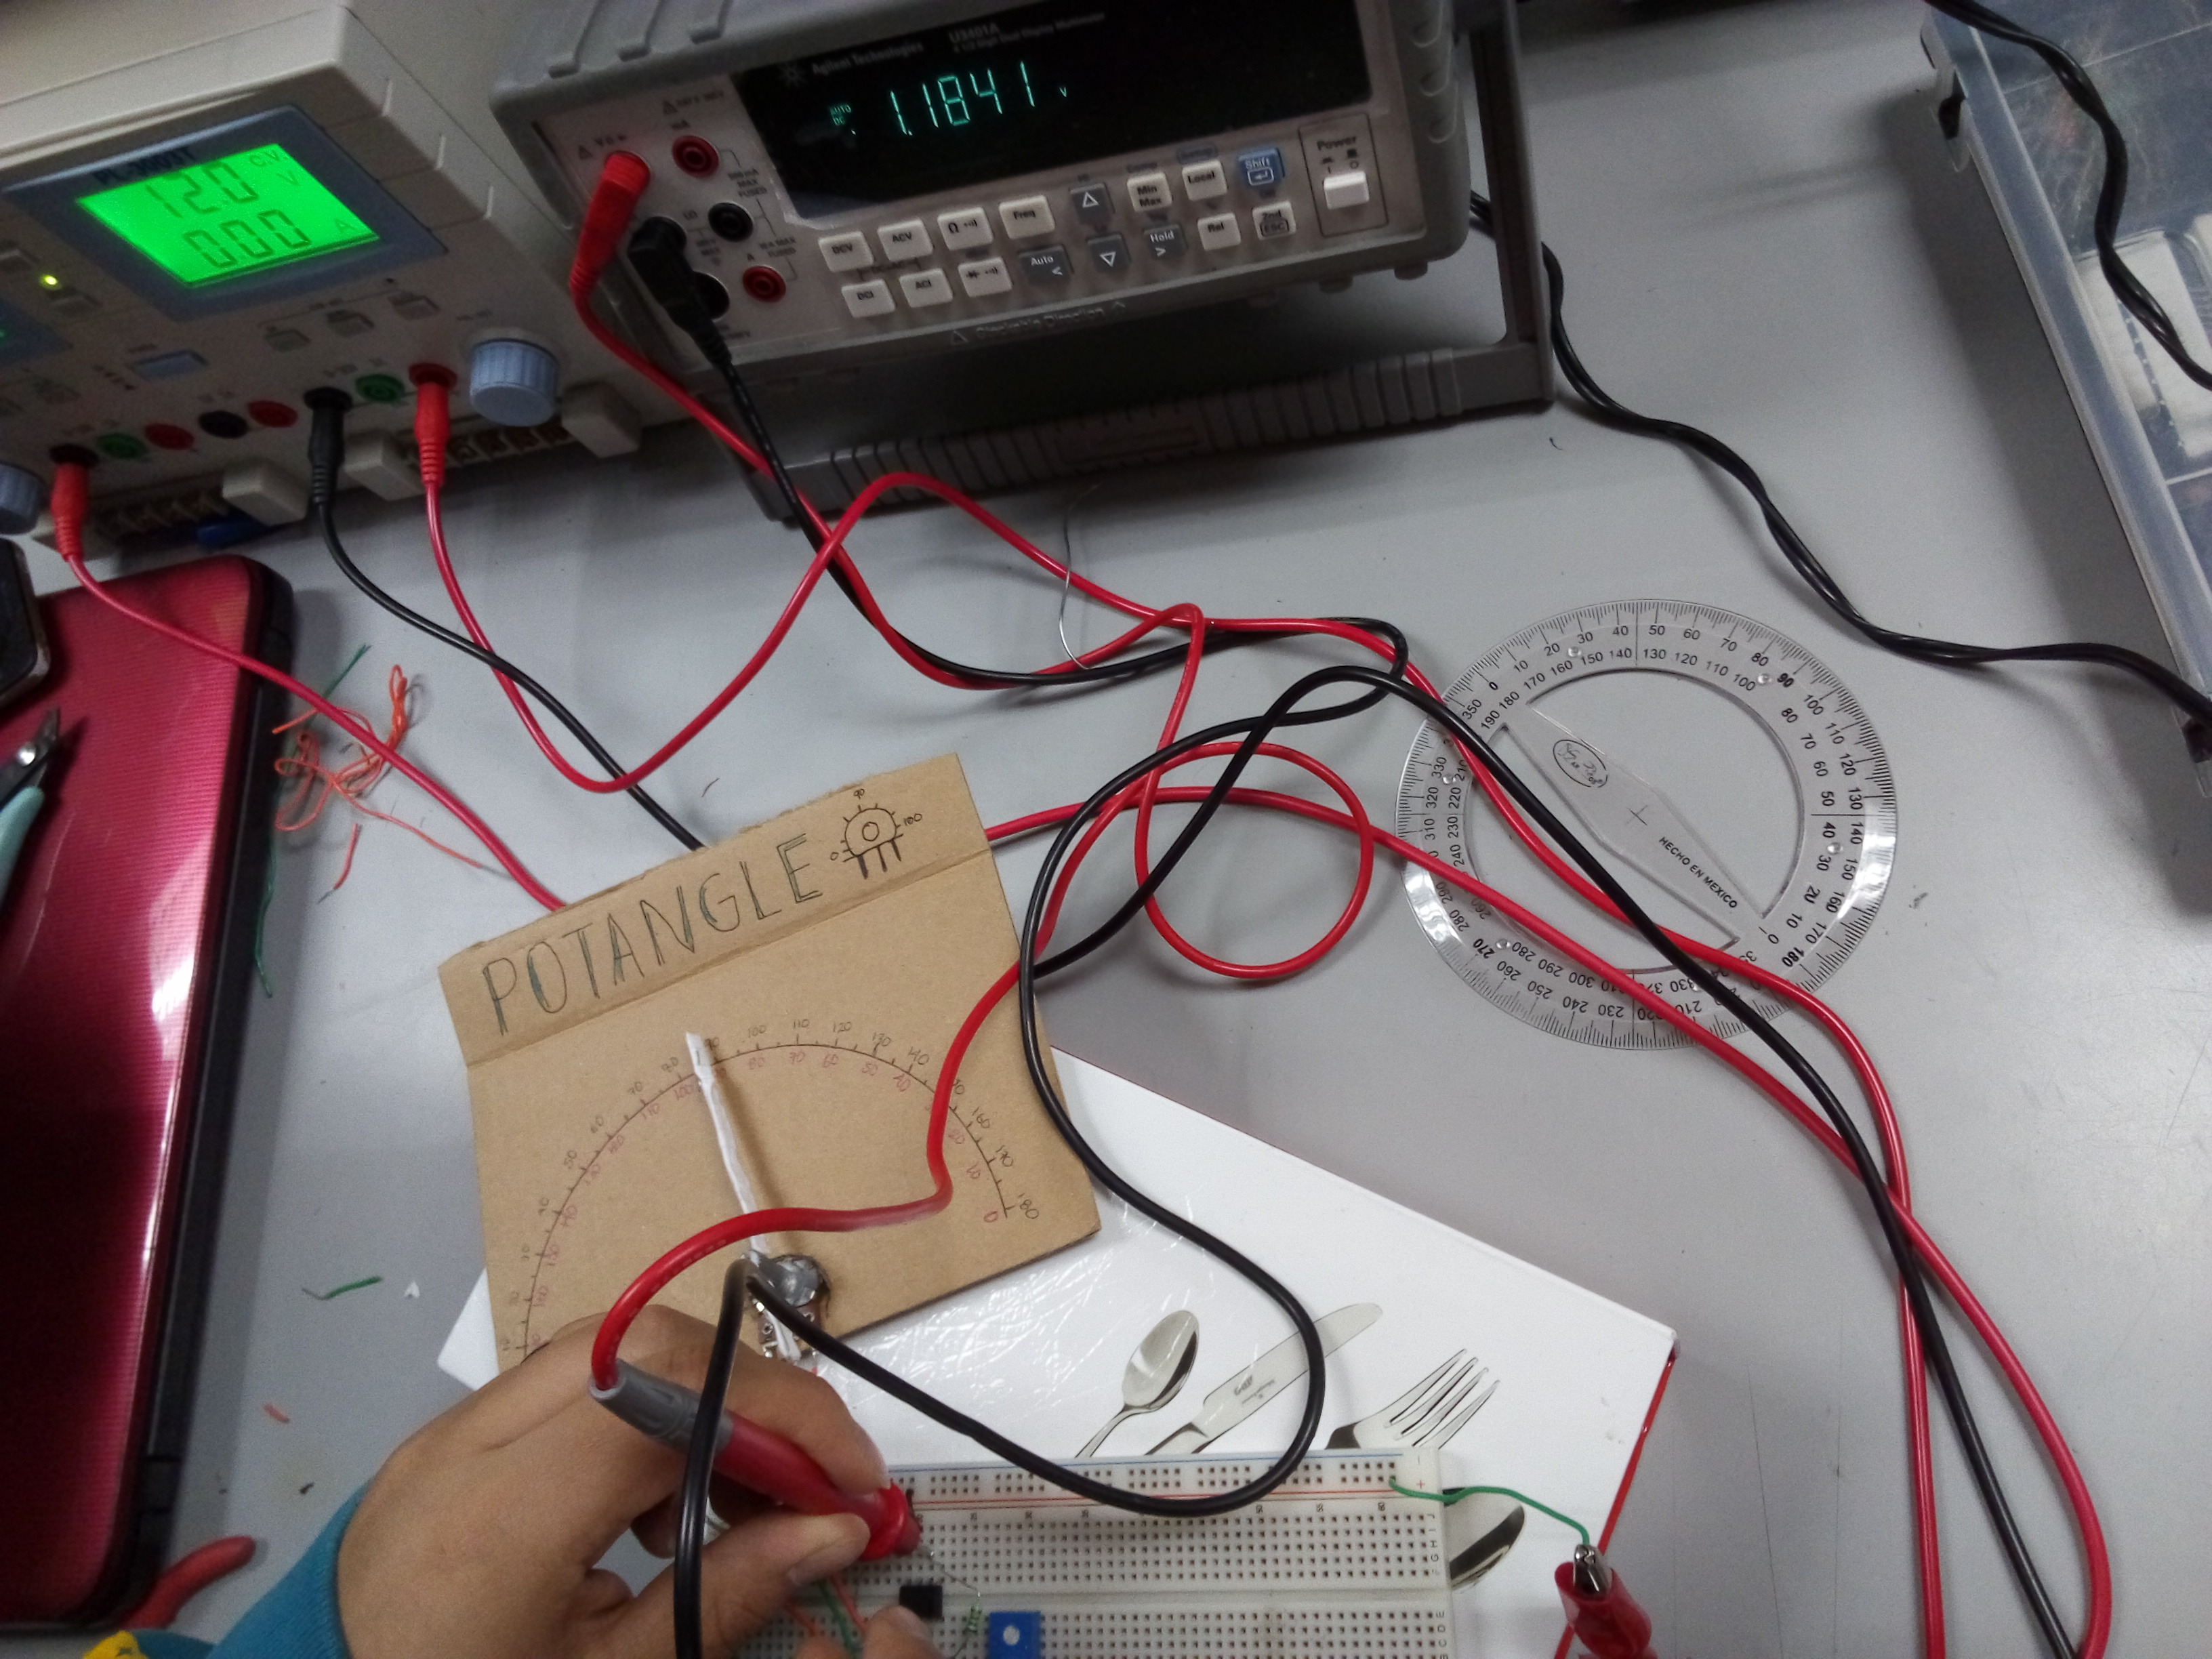
\includegraphics[width=0.8\textwidth]{Practica2/images/90grados.jpg}
            \end{figure}
            
        \textbf{Medida a 180 grados = 3.0051 V}
        \begin{figure}[h!]
                \centering
                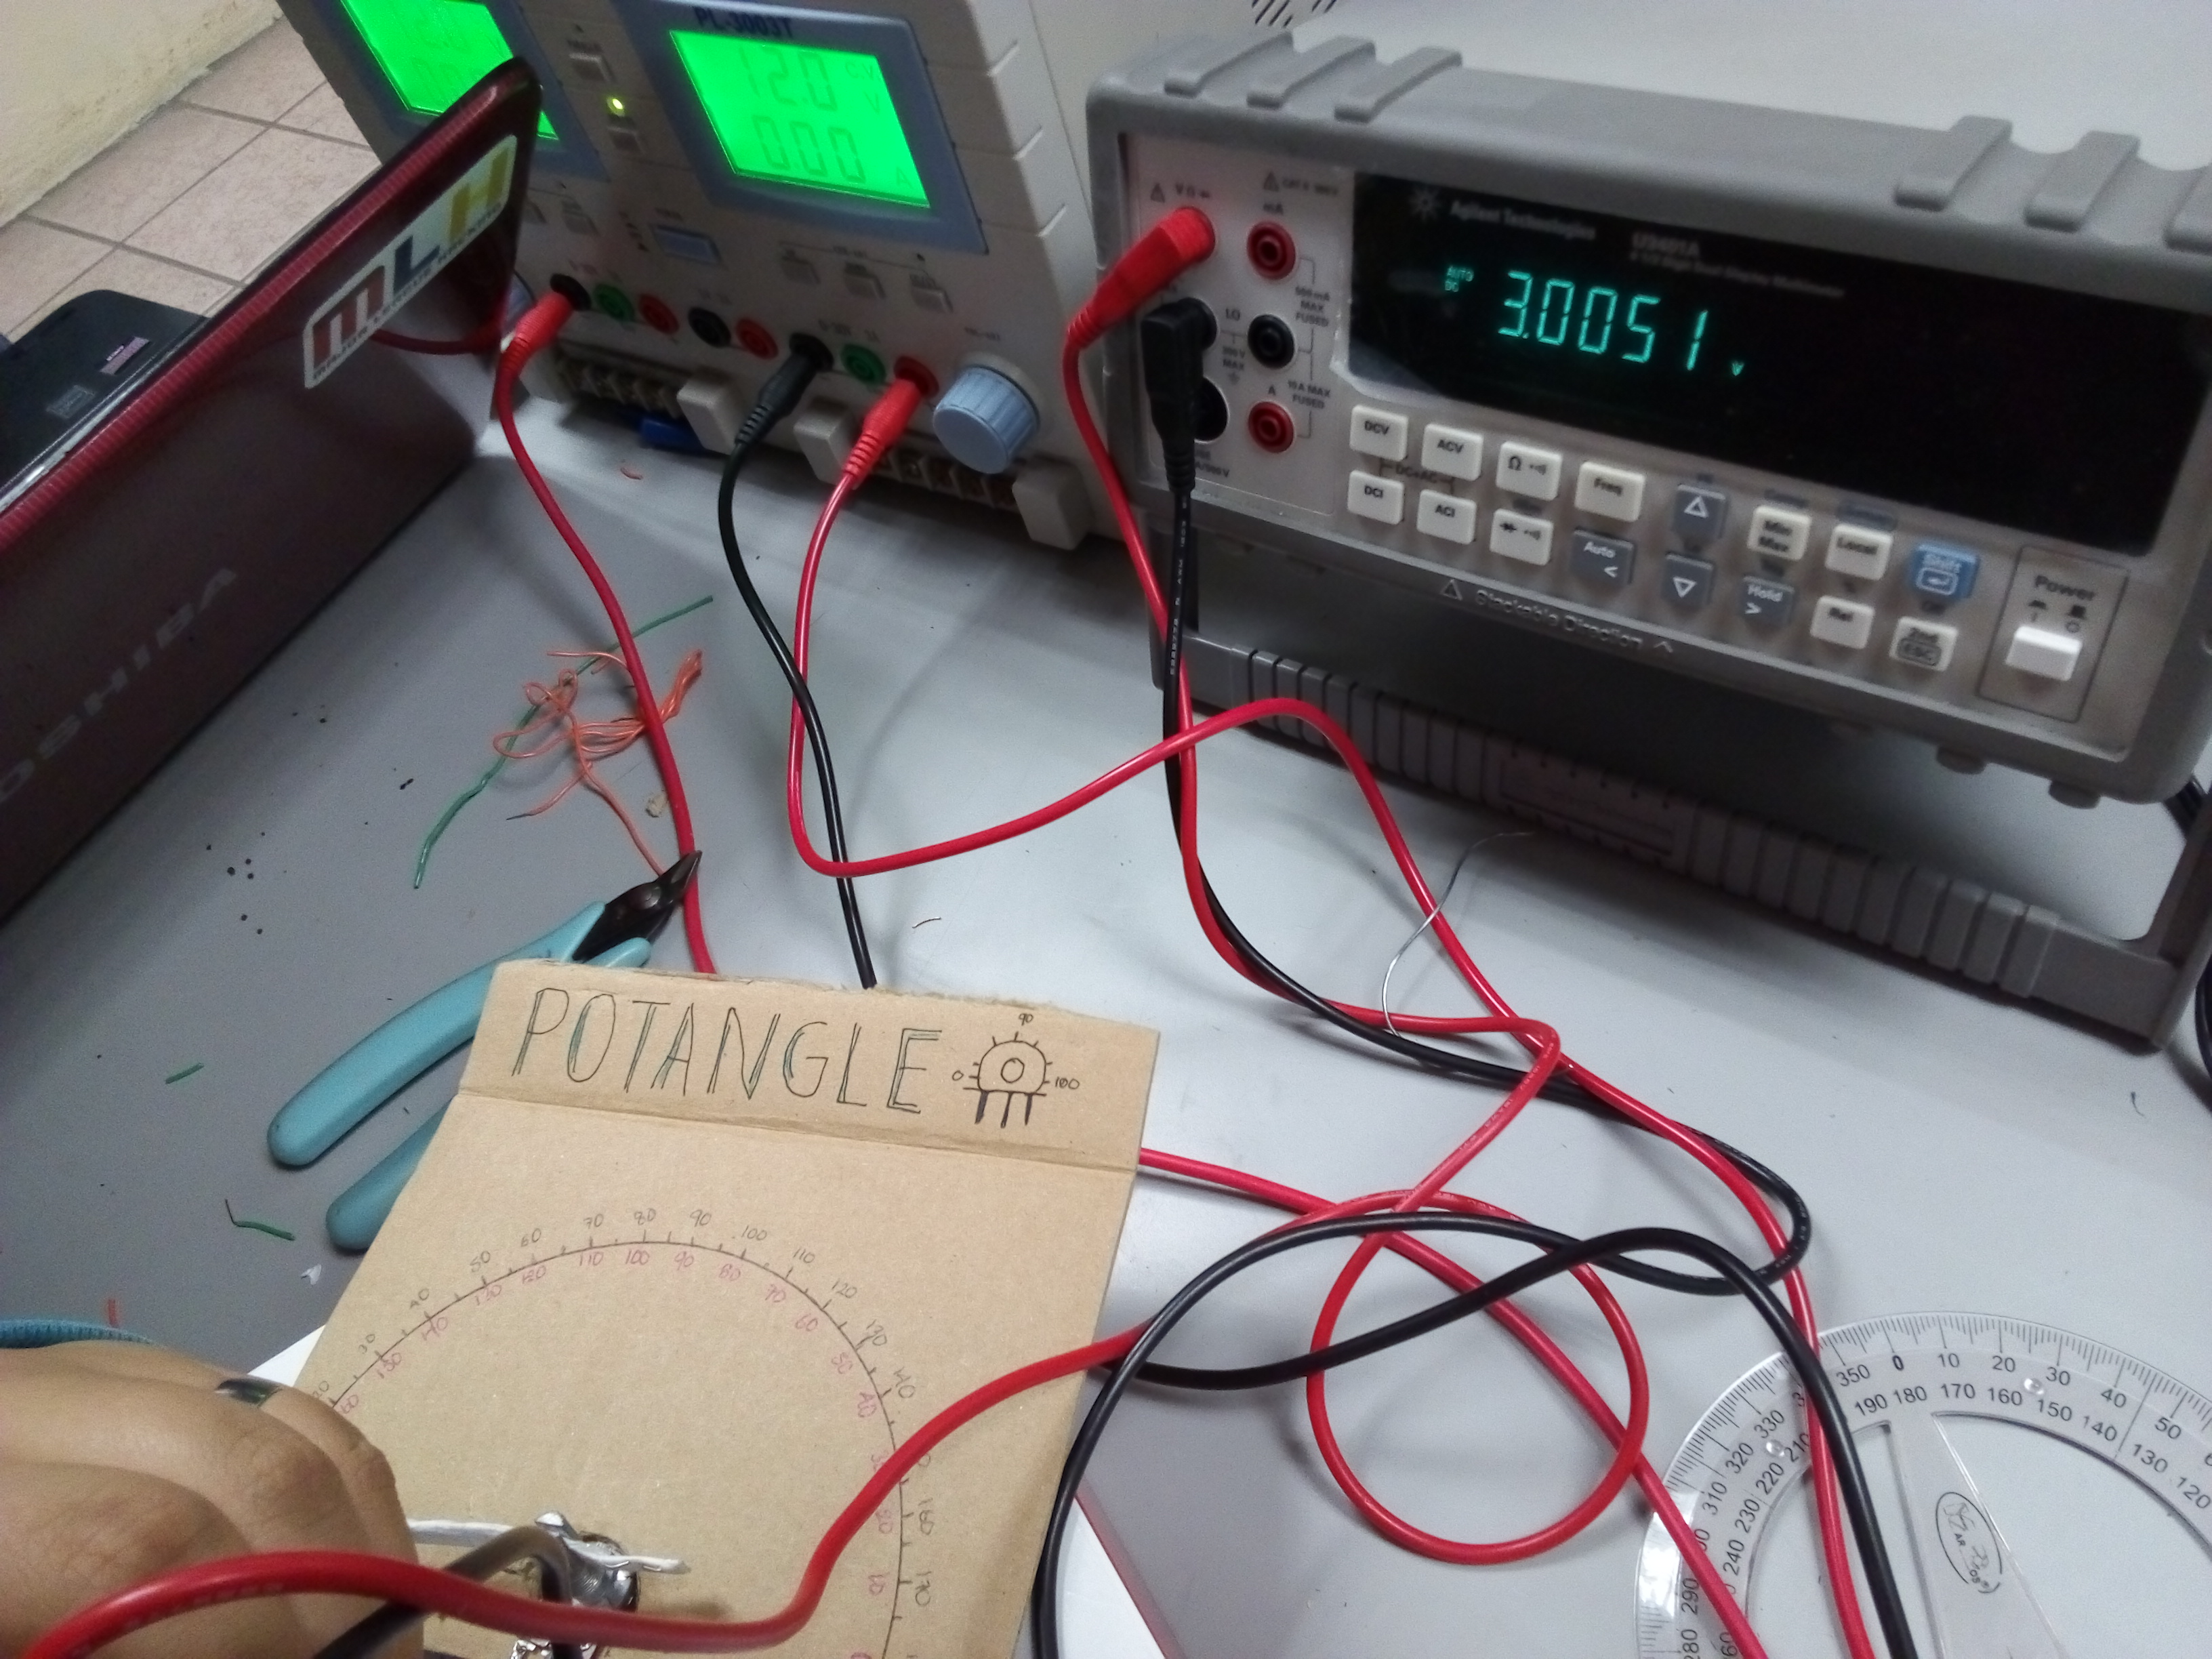
\includegraphics[width=0.8\textwidth]{Practica2/images/180grados.jpg}
            \end{figure}
        
    \newpage    
    \subsection{Página Web: POTANGLE}
    Diseñamos una página WEB muy sencilla para calcular de \textbf{grados} a \textbf{voltaje} con base en los cálculos mencionados anteriormente, cabe destacar que tal como se esperaba, existe un margen de error debido a que estamos aproximando. 
    
    \textbf{Pruébalo tu mismo con la siguiente url:} \\
    \url{https://abiisnn.github.io/INSTRU/Potangle/index.html}
    
    La página que nos aparecerá es la siguiente:
        \begin{figure}[h!]
                \centering
                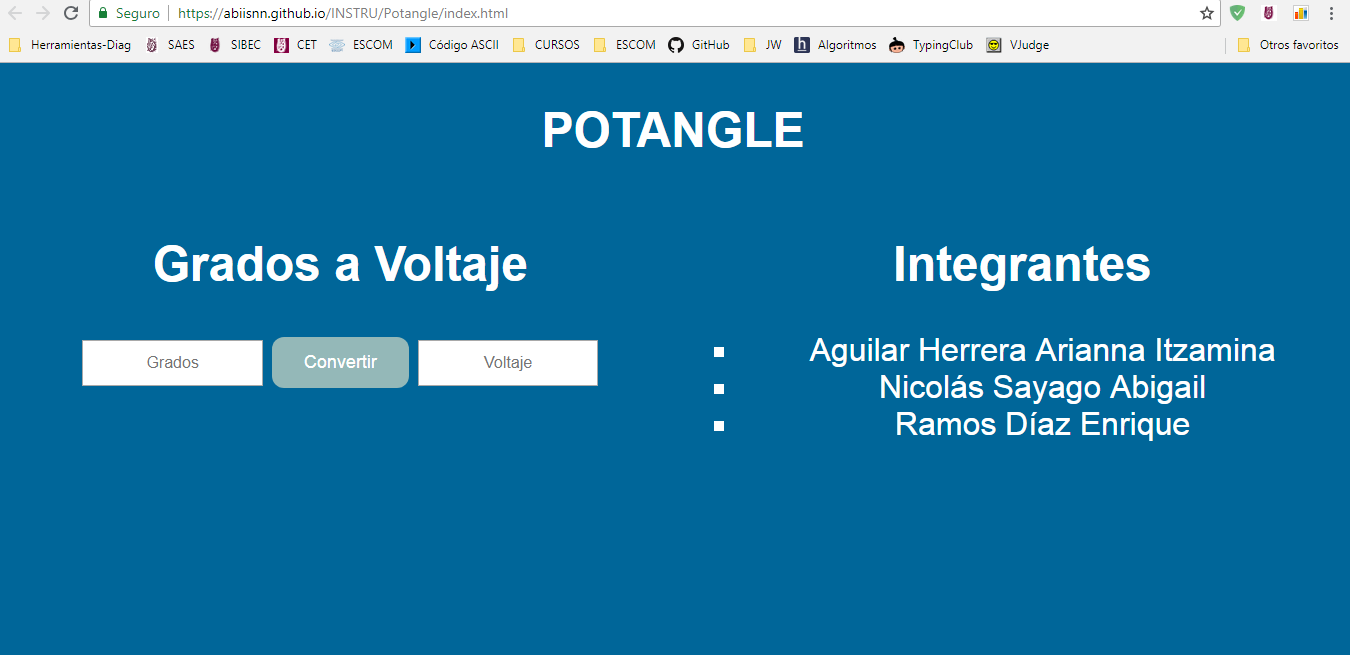
\includegraphics[width=\textwidth]{Practica2/images/po1.PNG}
    \end{figure}
    \\        
    Probamos el mismo ejemplo que hicimos en la sección anterior con los \textbf{100 grados} y observamos que el resultado es el correcto:
    
        \begin{figure}[h!]
                \centering
                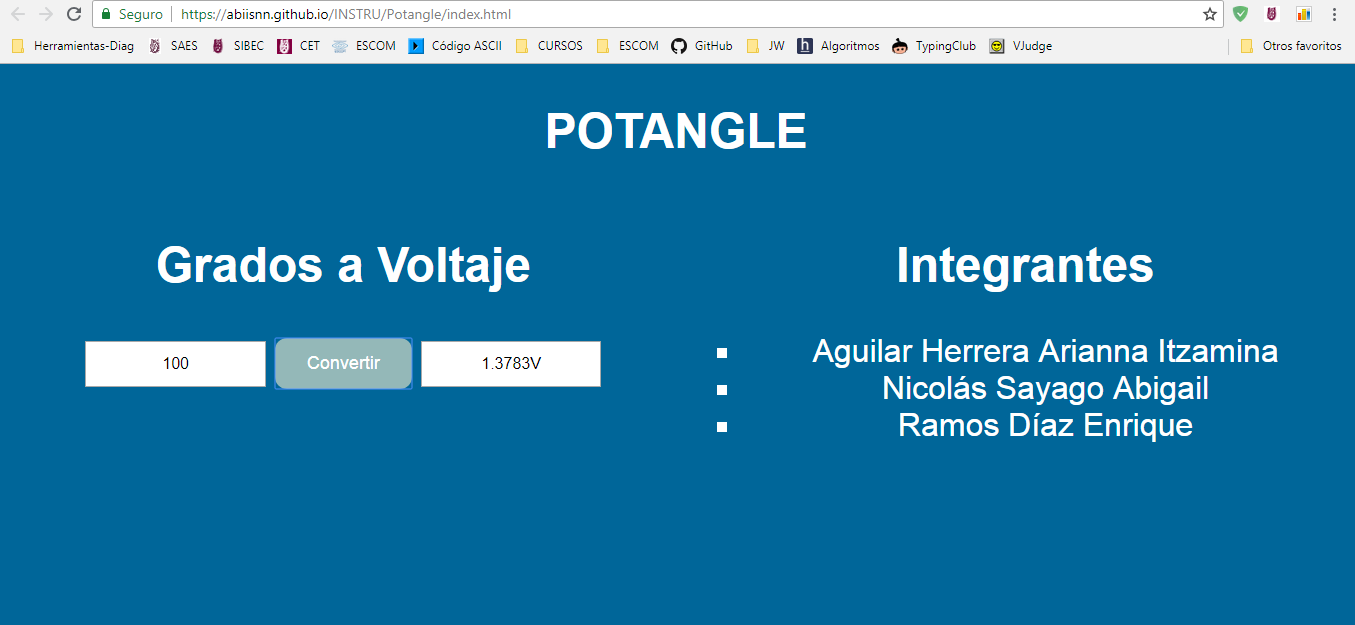
\includegraphics[width=\textwidth]{Practica2/images/po2.PNG}
            \end{figure}
    
    


	\newpage
	% /////////////////////////////////////////////////////////////////////
	%							CONCLUSIONES
	% ////////////////////////////////////////////////////////////////////
	\section{Conclusiones}
		\subsection{Aguilar Herrera Arianna Itzamina}
    En esta práctica ya se adentró más a lo que es propiamente instrumentación, pues en la materia se verán distintos tipos de sensores, en esta ocasión, se trabajó con un sensor potenciométrico, además de que se calculó todo el circuito, para así determinar los componentes que serían necesarios para el desarrollo de la práctica. 
    
    A lo largo de la práctica se observó que un sensor potenciométrico puede tener varios usos, se pudieron medir más variables, no solo se restringe a medir ángulos, también se repasó nuevamente el uso de los amplificadores no inversores.
    
    Pero puede que la parte más importante de esta práctica haya sido la retroalimentación, pues como se sabe, la retroalimentación es una parte importante de la instrumentación, regresar en lo ya establecido, hacer ajustes, para garantizar el funcionamiento del instrumento. 
    
		\subsection{Nicolás Sayago Abigail}
    Al finalizar esta práctica pude poner en práctica la teoría que ya conocía, por ejemplo el potenciómetro, anteriormente ya había trabajado con el, pero no sabía que se podía usar para hacer sensores sencillos, también el uso del amplificador que aunque recientemente lo usamos, nuevamente fue útil. 
    
    Cabe destacar que con ayuda de estos elementos pudimos hacer un sensor con su pequeña aplicación, en nuestro caso elegimos medir ángulos. Al realizar las mediciones notamos algunos detalles, nuestro pequeño diseño llamado \textbf{POTANGLE} no es exacto del todo, eso se debe a que al hacer la conversión en la página web, usamos un polinomio que solamente aproxima sus valores, sin embargo sigue siendo confiable. 
    
    Con respecto al armado del circuito, se tuvo algunos problemas por los valores que fuimos eligiendo, al hacer pruebas sucedía que al principio teníamos la medición de voltaje requerido pero bajaba.
    
    El valor práctico que en mi caso puedo tomar, es que es muy sencillo hacer este tipo de prácticas con pocos recursos y también combinar los conocimientos que ya tengo sobre la programación, teniendo como resultado un proyecto mejor planteado.
    
    
		\subsection{Ramos Díaz Enrique}
		A simple vista, el armado de esta práctica parecía sumamente sencillo, pues constaba en elementos básicos como resistencias, potenciómetros y amplificadores operacionales.
		
		Sin embargo, en la realización de esta surgieron un par de problemas:
		\begin{itemize}
		    \item Primero se propuso un rango en la intensidad de corriente de 4 a 20 mV, pero al momento de hacer los cálculos y diseño para la primera etapa, en donde nuestro potenciómetro era de $2k\Omega$, los valores de voltaje de la fuente de alimentación eran exageradamente altos, y además superaban los 5V que debía entregar la salida del amplificador. Para resolver esto, reducimos la corriente a solo 1mA
		    \item Al momento de añadir el regulador de voltaje LM7812 tuvimos un par de problemas al cablear los capacitores, pues no sabíamos que además de aquellos que van a cada entrada de +- 12 V de $10\mu F$, la hoja de especificaciones del 7812 indicada que también debían ir otros dos de $0.1\mu F$ extras [En la parte de anexo se explica más información al respecto]
		    \item A pesar de que el valor del potenciómetro indica $2k\Omega$, estos no eran reales, pues al cablear el diseño y medir el voltaje del potenciómetro este era de 1.86 V aproximadamente, y en amplificador operacional también daba problemas pues la salida no era de 5V, sino de 4.66V. Esto se solucionó con el cambio de la resistencia de $10k\Omega$ en el diseño por un preset del mismo valor y una resistencia de $1k\Omega$, para ajustar estos valores.
		    \item Cuando se realizaron las mediciones, se noto que el cursor del potenciómetro giraba más de una vuelta completa (360 grados) por lo que se tomo el valor más bajo como el inicio de nuestro rango (20 grados) y solo se midió hasta los 180 grados reales.
		\end{itemize}
		\newpage
	%/////////////////////////////////////////////////////////////////
	%							ANEXOS
	%/////////////////////////////////////////////////////////////////
	
	\section{Anexos}
	    \subsection{Alimentación del circuito}
	        Todos los amplificadores operacionales LM741 de los circuitos deben estar alimentados por una fuente de +12 V y -12 V en serie. [Consultar hoja de especificaciones del LM741 para más información]. Deben ir dos capacitores de $10\mu F$, uno por cada entrada de voltaje.
	        
	        \begin{figure}[h!]
                \centering
                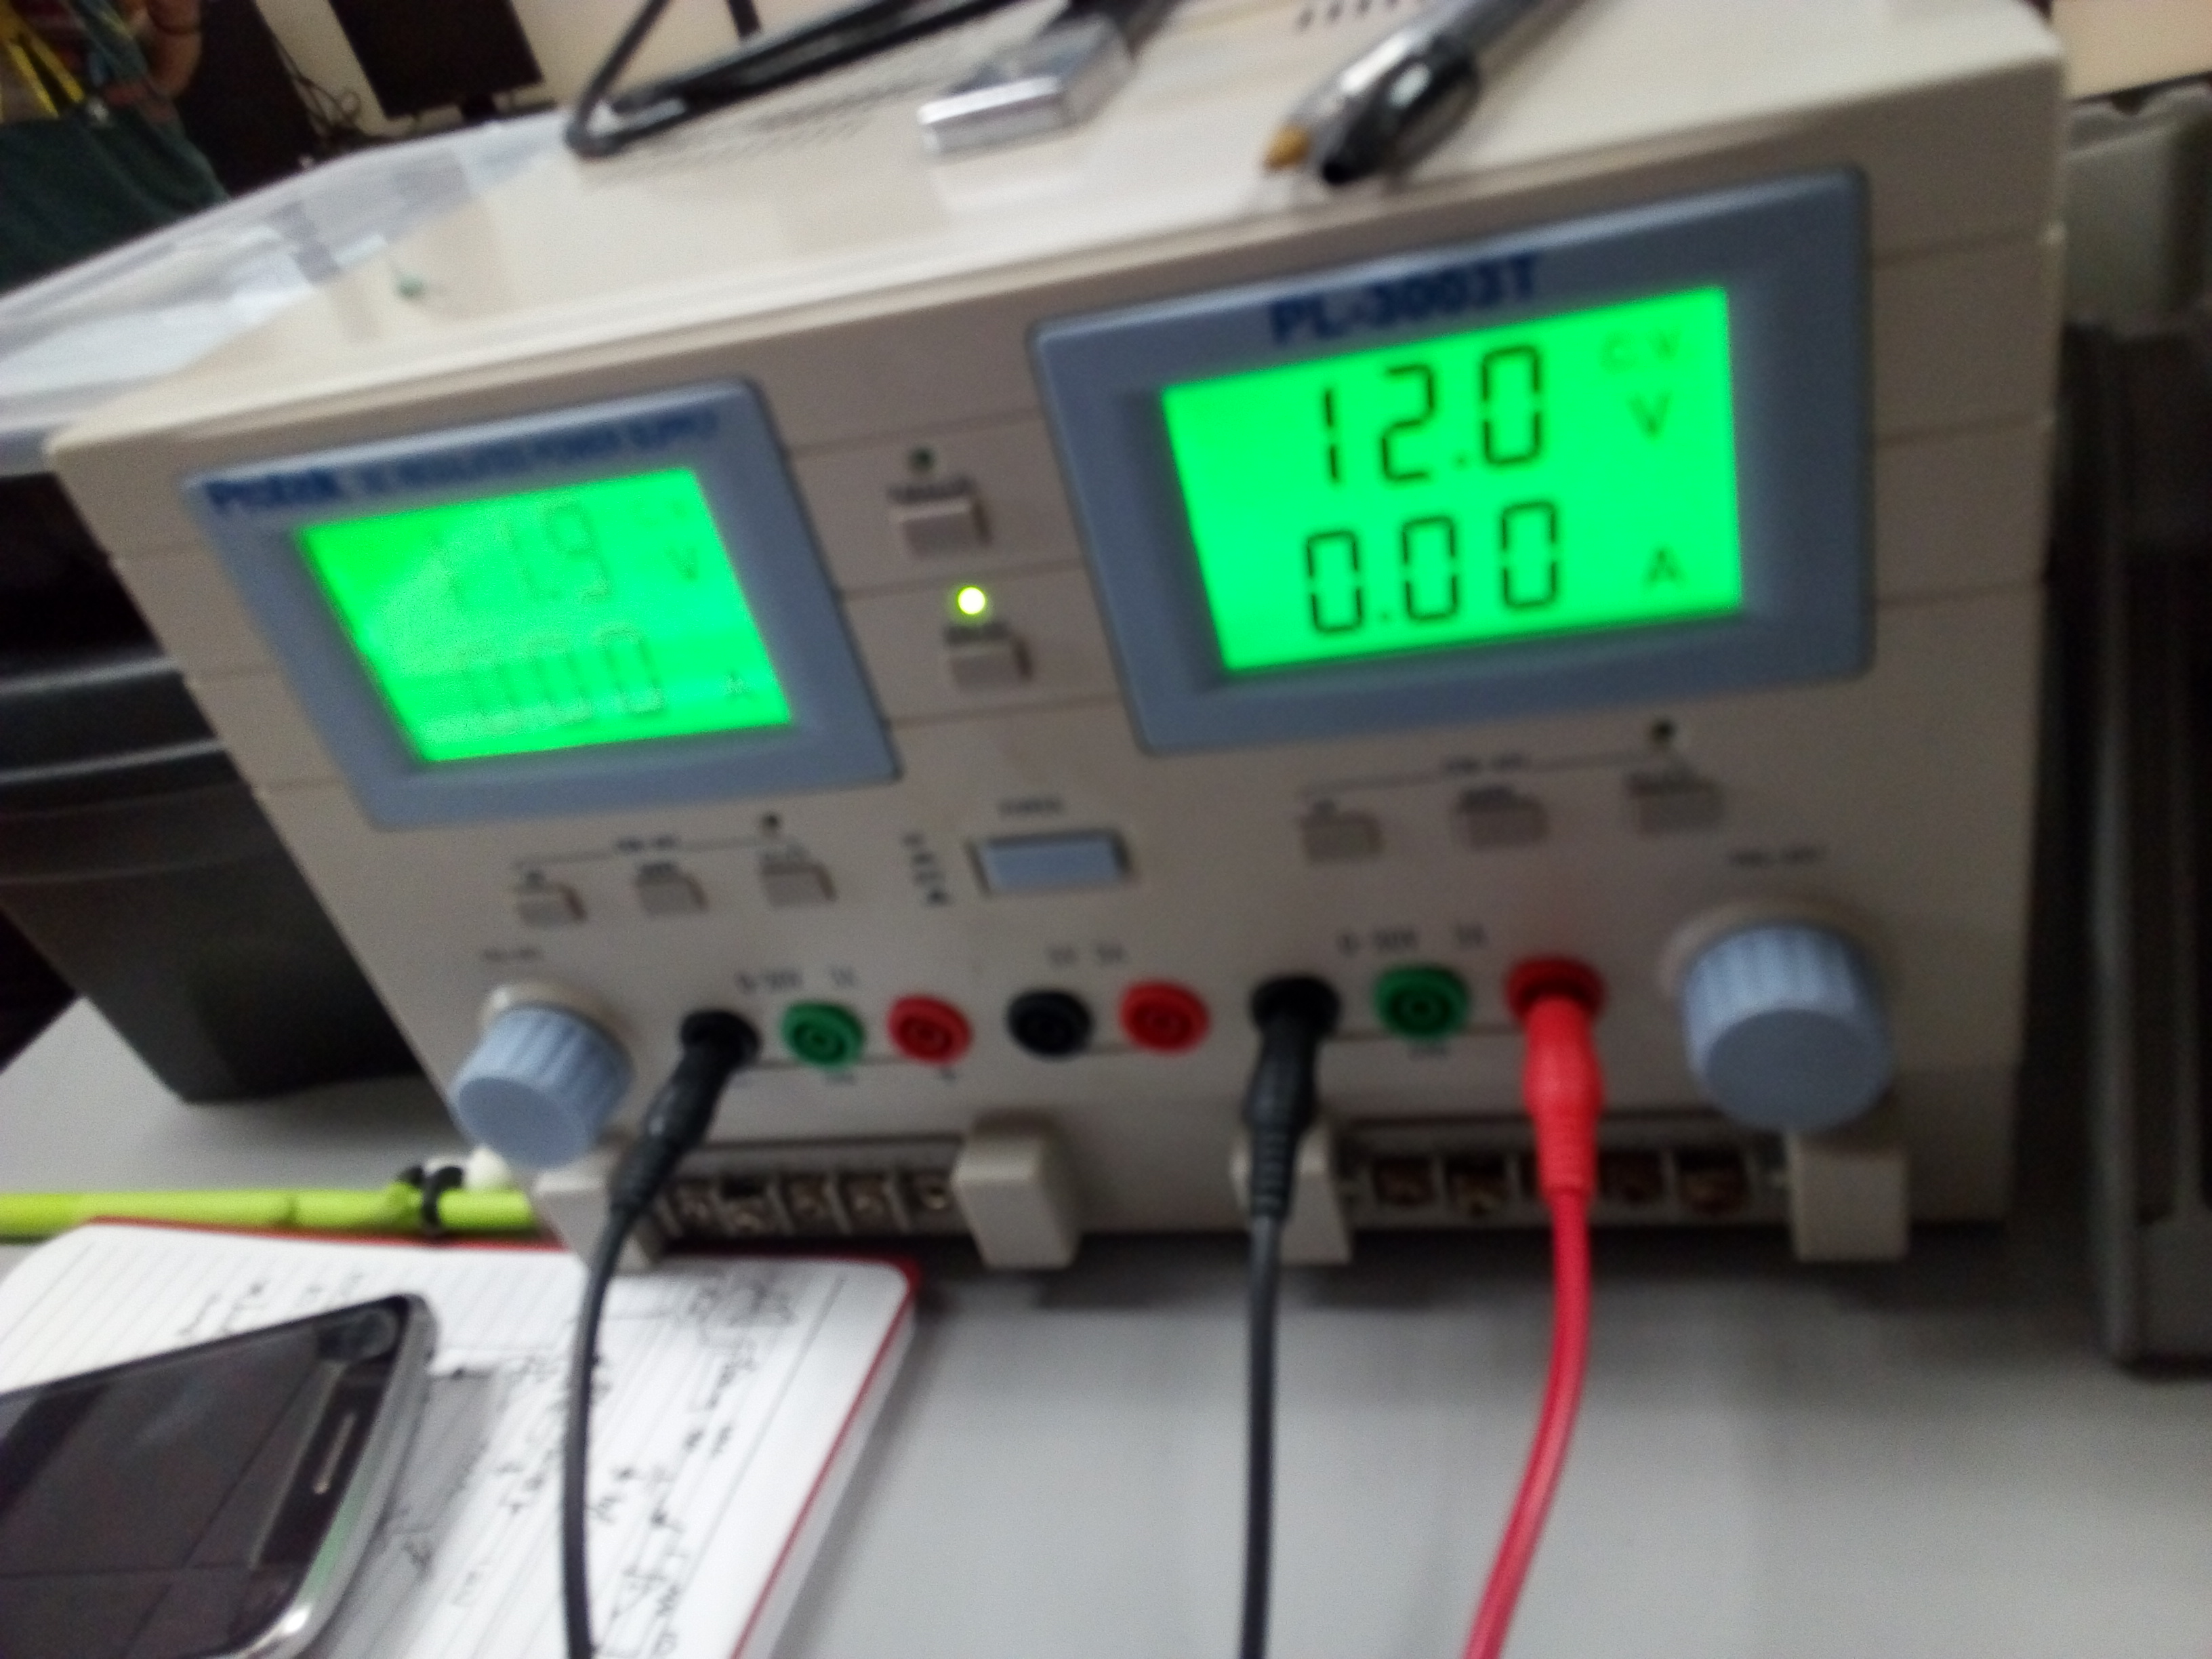
\includegraphics[width=0.7\textwidth]{Sismografo/Images/fuente.jpg}
            \end{figure} 
        \subsection{Configuración del regulador de voltaje LM7812}
        Es importante mencionar que en el regulador de voltaje LM7812, deben ir cableados dos capacitores de $0.1\mu F$, como se muestra en el siguiente esquema: [Consultar hoja de especificaciones del LM7812 para más información]
        
        \begin{figure}[h!]
                \centering
                \includegraphics[scale=1]{Practica2/images/7812.jpg}
            \end{figure}
        
            %/////////////////////////////////////////////////////////////////
	%                           REFERENCIAS
	%/////////////////////////////////////////////////////////////////

	\nocite{ref1, ref2, ref3, ref4}
	\bibliography{referencias}
        

	\end{document}
